\documentclass[10pt]{beamer}

\usepackage[utf8]{inputenc}
\usepackage{tcolorbox}
\usepackage{tikz}
\usepackage{tikz-3dplot}
\usetikzlibrary{intersections,calc,,angles,quotes,through}
\usepackage{amsmath}
\usepackage{graphicx}
\usepackage{cases}
\def \heart {\textcolor{blue}{$\heartsuit$} }
\def \C {\mathcal{C}}
\def \orthog {\underline{\perp}}
\def\arcos{\operatorname{arcos}}
\def \deg {^{\circ}}

\newcommand{\vect}[1] {
  \overrightarrow{#1}}

\tcbset{%
	basic/.style={colframe=black,
		      colback=white,
		      top= 0mm,
		      bottom = 2mm,
		      boxsep=0mm
		      }
}
\tikzset{
    invisible/.style={opacity=0},
    visible on/.style={alt={#1{}{invisible}}},
    alt/.code args={<#1>#2#3}{%
      \alt<#1>{\pgfkeysalso{#2}}{\pgfkeysalso{#3}} % \pgfkeysalso doesn't change the path
    },
  }

    
\begin{document}  
    \beamertemplatenavigationsymbolsempty
    \setlength{\abovedisplayskip}{0pt}
    \setlength{\belowdisplayskip}{0pt}
    \frame{
	  
	  \frametitle{Exercice sur les points particuliers du triangle. }
	  %\renewcommand{\theenumi}{\alph{enumi})}
	  Dans un triangle $ABC$, montrer que \\
	  $$3\vect{OG}=\vect{OH}$$  \\
	  
	  si $O$ est le centre du cercle circonscrit au triangle, $G$ son
	  centre de gravité et $H$ son orthocentre.
	  \vfill
	  
	  \pause
	  % hypothèses et thèse
	  \begin{tcolorbox}[basic] 
	      \begin{columns}[t]
		 
		 \column{.5\textwidth}\centering
		      
		      \underline{Hypothèses} 
		      \begin{itemize}
		      \item $G$ centre de gravité,
		      \item $H$ orthocentre.
		      \end{itemize}

		  
		  \column{.5\textwidth}\centering
		      
		      \underline{Thèse} \\
		      \smallskip
		      $3\vect{OG}=\vect{OH}$.
		
	      \end{columns}
	  \end{tcolorbox}
    }

    \frame{ 
	  % résolution ex1
	  \begin{columns}[t]
		\column{.5\textwidth}\centering 
		

			\underline{Dessin}\\
				  \vspace{-15mm}
				  \begin{figure}[h]
				  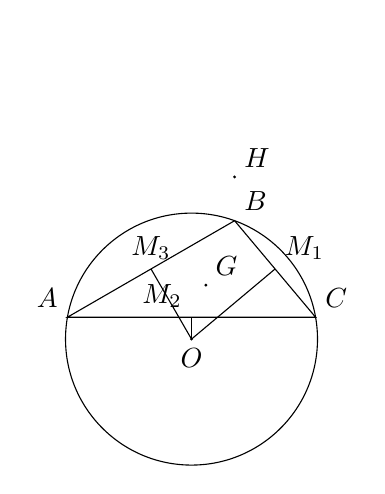
\begin{tikzpicture}[scale=0.8]
			          %projection ($(X)!(B')!(B)$)
			          %nommer chemin 'name path
			          %intersection \path [name intersections={of=d and gb,name=G}];
			          %animation  \draw[visible on=<1>] 
				  %           \draw[visible on=<{2,4}>]
				  %angle arc[radius = 6mm, start angle= 180, end angle= 225] node [below left,pos=0.3]{$\alpha$}
				  %angle \pic [draw,"$\alpha$", angle eccentricity=1.5] {angle = A'--A--B};
				  %perpendiculaire ($(A')!3cm!-90:(A)$)
				  %cercle par point \node [draw] at (A) [circle through=(B)] {};
				  
				  %CERCLE et triangle
				  \coordinate[label=below:$O$] (O) at (0,0);
				  \coordinate[label=above right:$B$] (B) at (70:2);
				  \coordinate[label=above right:$C$] (C) at (10:2);
				  \coordinate[label=above left:$A$] (A) at (170:2);
				  \draw[name path =cercle] (O) circle (2);
				  \draw (A) -- (B)--(C) --cycle;
				  \fill (O) circle (0.025);
				  
				  %G
				  \coordinate[label=above right:$G$] (G) at ($.333*(A)+.333*(B)+.333*(C)$);
				  \fill (G) circle (0.025);
				  %H
				  \path[name path=BH] (B) -- +($2*(B)-2*(A)!(B)!(C)$);
				  \path[name path=CH] (C) -- +($2*(A)!(C)!(B)-2*(C)$);
				  \path [name intersections={of=BH and CH,by=H}];
				  \coordinate[label=above right:$H$] () at (H);
				  \fill(H) circle (0.025);
				  %M_1,M_2,M_3
				  \coordinate (M_1) at ($(B)!.5!(C)$);
				  \draw[visible on=<2>] (O) -- (M_1) node[above right] {$M_1$};
				  
				  \coordinate (M_2) at ($(A)!.5!(C)$);
				  \draw[visible on=<3>] (O) -- (M_2) node[above left] {$M_2$};
				  
				  \coordinate (M_3) at ($(A)!.5!(B)$);
				  \draw[visible on=<4>] (O) -- (M_3) node[above] {$M_3$};
				  \end{tikzpicture}
				  \end{figure}
			
				  \begin{tcolorbox}[basic] 
				      
				    \smallskip
				    \underline{Hypothèses} 
				    \begin{enumerate}
				    \item $G$ centre de gravité,
				    \item $H$ orthocentre.
				    \end{enumerate}
							      
				    \underline{Thèse} \\
				    \smallskip
				    $3\vect{OG}=\vect{OH}$.
				    \end{tcolorbox}
		
		
		\column{.5\textwidth}\centering
		
		\underline{Résolution}\\ \flushleft
		
		\onslide<+->\begin{enumerate}
			    \item $\vect{OG} = \frac{1}{3}\ \vect{OA} + \frac{1}{3}\ \vect{OB} + \frac{1}{3}\ \vect{OC}$, \\[1em]
			    \item $\vect{AH}\cdot\vect{BC}=0$, \\[0.5em]
				  $\vect{BH}\cdot\vect{AC}=0$, \\[0.5em] 
				  $\vect{CH}\cdot\vect{AB}=0$.
			    \end{enumerate}	\bigskip
		
		Avec $\vect{OP}=3\ \vect{OG}$, la thèse devient : \\ \medskip
		$\vect{OP}=\vect{OH}$. $ie.\ P=H.$ \\ \bigskip
		\vspace{-4mm}
		\onslide<+->\begin{align*}
			    \vect{AP}=\vect{AO}+\vect{OP}=\ & \vect{OB}+\vect{OC}, \\[0.3em]
							 =\ & 2\ \vect{OM_1} + \vect{M_1B} + \vect{M_1C}, \\[0.3em]
							 =\ & 2\ \vect{OM_1}.
			    \end{align*} 
		\smallskip	    
		
		\onslide<+->De la même façon, \\ \medskip
		$\vect{BP}= 2\ \vect{OM_2}$, \onslide<+-> $\vect{CP}= 2\ \vect{OM_3}$.
		
		
	
					
		
		\bigskip
		
		
		%\centering\noindent\rule{2cm}{0.4pt}
	   \end{columns} 
    }
    \frame{ 
	  % résolution ex1
	  \begin{columns}[t]
		\column{.5\textwidth}\centering 
		

			\underline{Dessin}\\
				  \vspace{-15mm}
				  \begin{figure}[h]
				  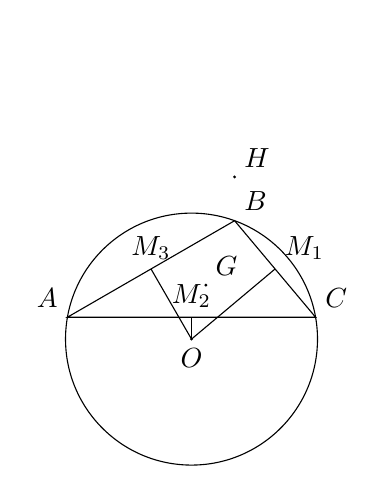
\begin{tikzpicture}[scale=0.8]
			          %projection ($(X)!(B')!(B)$)
			          %nommer chemin 'name path
			          %intersection \path [name intersections={of=d and gb,name=G}];
			          %animation  \draw[visible on=<1>] 
				  %           \draw[visible on=<{2,4}>]
				  %angle arc[radius = 6mm, start angle= 180, end angle= 225] node [below left,pos=0.3]{$\alpha$}
				  %angle \pic [draw,"$\alpha$", angle eccentricity=1.5] {angle = A'--A--B};
				  %perpendiculaire ($(A')!3cm!-90:(A)$)
				  %cercle par point \node [draw] at (A) [circle through=(B)] {};
				  
				  %CERCLE et triangle
				  \coordinate[label=below:$O$] (O) at (0,0);
				  \coordinate[label=above right:$B$] (B) at (70:2);
				  \coordinate[label=above right:$C$] (C) at (10:2);
				  \coordinate[label=above left:$A$] (A) at (170:2);
				  \draw[name path =cercle] (O) circle (2);
				  \draw (A) -- (B)--(C) --cycle;
				  \fill (O) circle (0.025);
				  
				  %G
				  \coordinate[label=above right:$G$] (G) at ($.333*(A)+.333*(B)+.333*(C)$);
				  \fill (G) circle (0.025);
				  %H
				  \path[name path=BH] (B) -- +($2*(B)-2*(A)!(B)!(C)$);
				  \path[name path=CH] (C) -- +($2*(A)!(C)!(B)-2*(C)$);
				  \path [name intersections={of=BH and CH,by=H}];
				  \coordinate[label=above right:$H$] () at (H);
				  \fill(H) circle (0.025);
				  %M_1,M_2,M_3
				  \coordinate (M_1) at ($(B)!.5!(C)$);
				  \draw (O) -- (M_1) node[above right] {$M_1$};
				  
				  \coordinate (M_2) at ($(A)!.5!(C)$);
				  \draw (O) -- (M_2) node[above] {$M_2$};
				  
				  \coordinate (M_3) at ($(A)!.5!(B)$);
				  \draw (O) -- (M_3) node[above] {$M_3$};
				
				  \end{tikzpicture}
				  \end{figure}
			
				  \begin{tcolorbox}[basic] 
				      
				    \smallskip
				    \underline{Hypothèses} 
				    \begin{enumerate}
				    \item $G$ centre de gravité,
				    \item $H$ orthocentre.
				    \end{enumerate}
							      
				    \underline{Thèse} \\
				    \smallskip
				    $3\vect{OG}=\vect{OH}$.
				    \end{tcolorbox}
		
		
		\column{.5\textwidth}\centering
		
		\underline{Résolution}\\ \flushleft
		
		$\begin{cases}
		 \vect{AP}= 2\ \vect{OM_1}, \\
		 \vect{BP}= 2\ \vect{OM_2}, \\ 
		 \vect{CP}= 2\ \vect{OM_3}. \\
		\end{cases}$ \\ \bigskip
		\heart La droite passant par le centre d'un cercle et le milieu d'une de ses cordes est perpendiculaire à cette corde. \\ \bigskip
		$\vect{AP}\cdot\vect{BC}=0$, \\[0.5em]
	        $\vect{BP}\cdot\vect{AC}=0$, \\[0.5em] 
	        $\vect{CP}\cdot\vect{AB}=0$. \\ \bigskip
	        $P=AH\cap BH\cap CH \rightarrow P=H$. \hfill $\qed$
		
		
		
	
					
		
		\bigskip
		
		
		%\centering\noindent\rule{2cm}{0.4pt}
	   \end{columns} 
    }
  
\end{document}
